\section{Proposta}

Este trabalho tem como proposta a utilização de um modelo de inteligência artificial para segmentação de imagem e permitir os usuários gerarem mapas a partir da seleção de um dos segmentos da imagem.

Utilizando o modelo de rede neural totalmente convolucional é possível fazer a segmentação panóptico da imagem da seguinte forma:

\begin{figure}[!ht]
	\centering
    \caption{Imagem de entrada para rede neural.}
	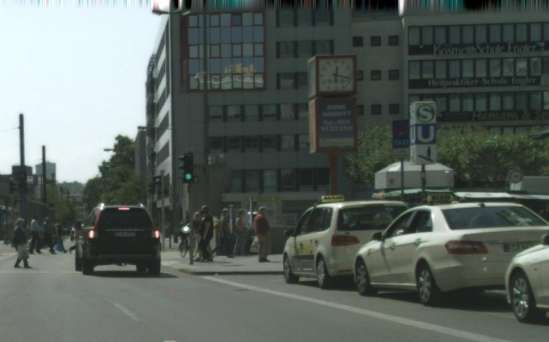
\includegraphics[width=0.6\textwidth]{figures/segmantations_1.png}
    \legend{Fonte: \citeonline{kirillov2019panoptic}}
	\label{fig:segmantations_1}
\end{figure}

\begin{figure}[!ht]
	\centering
    \caption{Imagem segmentada de saída da rede neural totalmente convolucional de segmentação panóptico.}
	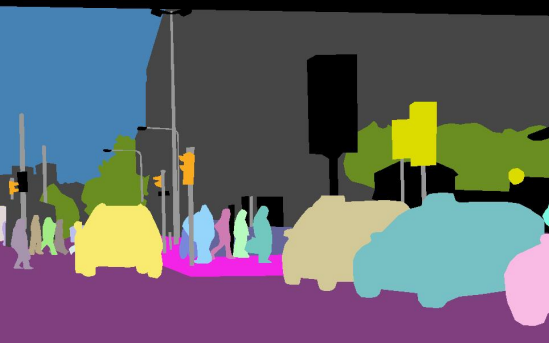
\includegraphics[width=0.6\textwidth]{figures/segmantations_2.png}
    \legend{Fonte: \citeonline{kirillov2019panoptic}}
	\label{fig:segmantations_2}
\end{figure}

Após a segmentação da imagem o usuários poderá selecionar qual parte da imagem sera utilizada para gerar a ilha.

Feito a seleção sera gerado um diagrama de Voronoi que irá funcionar como um filtro em cima dessa imagem e assim gerando a ilha e os biomas.

\begin{figure}[!ht]
	\centering
    \caption{Ilha gerada a partir da segmentação de imagem e aplicando um filtro com o diagrama de Voronoi, azul representa oceano, verde floresta, cinza montanhas.}
	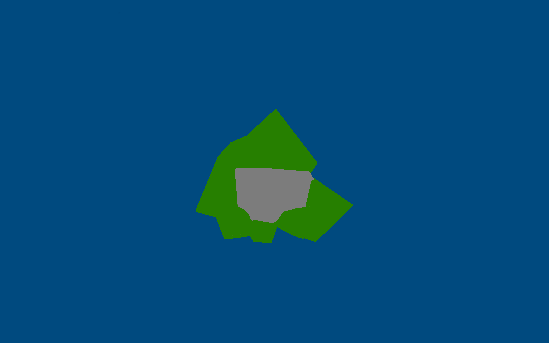
\includegraphics[width=0.6\textwidth]{figures/segmantations_pnl.png}
    \legend{Fonte: Criação propria}
	\label{fig:segmantations_pnl}
\end{figure}

